\documentclass[unnumsec,webpdf,contemporary,large]{oup-authoring-template}
\usepackage{booktabs}
\usepackage{longtable}
\usepackage{array}
\usepackage{float}
\usepackage{setspace}
\graphicspath{{figures/}}
\newcommand{\visiblealt}[1]{\figalttext{Alt text: #1}\par\smallskip\noindent{\small\textbf{Alt text:} #1}\par}
\begin{document}
\doublespacing
\renewcommand{\thetable}{S\arabic{table}}
\renewcommand{\thefigure}{S\arabic{figure}}

\journaltitle{Journal of the American Medical Informatics Association}
\DOI{To be assigned}
\copyrightyear{2026}
\pubyear{2026}
\vol{XX}
\issue{x}
\access{To be assigned}
\appnotes{Supplementary Material}
\firstpage{1}

\title[Supplementary material]{Supplementary Material for: From Clinician-Facing Narrative to Patient-Facing Instructions: How Stigmatizing Language Differs Across Clinical Notes}
\abstract{Supplementary methods, LLM verification of disease cohorts, complete primary binary results, sensitivity analyses, and reproducibility requirements.}
\keywords{supplementary material}
\maketitle
\onecolumn

\section{Supplementary Methods}

\subsection{Section parsing and cohort construction}

Discharge Instructions (DI) was defined as the patient-facing section, while the remaining discharge-summary sections were classified as clinician-facing. The empirical analyses compared DI with Brief Hospital Course (BHC) as the primary clinician-facing section and History of Present Illness (HPI) as a secondary clinician-facing section. Discharge summaries were segmented at curated headers occurring at the start of a line, with adjacent headers delimiting a section body. The primary cohort required both BHC and DI, with at least 50 tokens in each. HPI was included only in its separate paired comparison. The parser scanned 331,793 notes, found 290,005 with both primary sections, and retained 259,207 after the length threshold. Header rules, token definition, and the full cohort flow are given in the Supplementary Note (Section~\ref{sec:s_processing}).

The group-analysis build linked every retained note to note-level subject and admission identifiers. Twenty notes had no matching HOSP patient or admission record and lacked sex and age; complete-case modeling excluded these notes. The final group-analysis cohort contained 259,187 notes, 259,187 admissions, 125,271 subjects, and 518,374 paired BHC and DI rows. Missing insurance was coded as non-Medicaid for 2,793 notes. Missing language was coded as English or LEP=0 for 398 notes. These were coding decisions rather than row exclusions.

\subsection{LLM verification of ICD-coded disease cohorts}

Disease cohorts were defined from ICD diagnosis codes linked to each admission. Because a diagnosis code does not guarantee that the condition is documented in the discharge summary, we assessed whether each coded condition was supported by the note text. Each admission--disease pair was adjudicated independently by five open-weight large language models (LLMs): Qwen3.5-27B, Gemma-4-31B, GLM-4-32B, Mistral-24B, and gpt-oss-20b. Each model read seven sections of the discharge summary, with BHC, DI, HPI, Social History, and the ICD codes withheld (Supplementary Note), and returned one of three labels: SUPPORTED, REFUTED, or INSUFFICIENT. The adjudication covered 164,770 admission--disease pairs from 122,301 admissions across eight disease cohorts, for 823,850 model inferences. Outputs that could not be parsed were treated as missing votes rather than as a label: 568 for gpt-oss-20b (0.345\%), 67 for GLM-4-32B (0.041\%), 15 for Mistral-24B (0.009\%), 1 for Gemma-4-31B (0.001\%), and none for Qwen3.5-27B, totaling 651 (0.079\%).
% TODO(HY): add the prompt summary, label definitions, decoding settings, and the SUPPORTED-vote threshold used to define the analytic disease cohorts.

Agreement was summarized for the three labels and for a binary collapse of SUPPORTED versus REFUTED or INSUFFICIENT. Overall agreement across the five models used Fleiss \(\kappa\), Krippendorff \(\alpha\), which accommodates missing ratings, and the proportion of pairs on which all five models agreed. Pairwise agreement was calculated for each of the 10 model pairs. Results were stratified by disease and by the position of the qualifying code in the admission's diagnosis sequence: principal (sequence number 1), middle (2--9), and late (10 or higher). To assess how verification affected disease modification, we refitted the Layer 3 model with disease cohorts restricted to admission--disease pairs with at least three, or all five, SUPPORTED votes and compared the resulting interaction RRs with those from the unverified ICD-coded cohorts.

\subsection{Training data}

Classifier training used the Harrigian annotation resource and 89-keyword lexicon. The binary target combined negative, disbelief, and difficult annotations as stigma; positive, neutral, and exclude annotations formed non-stigma. The 5,043 examples were split by note identifier into 4,037 training, 501 validation, and 505 test examples. Primary input contained the keyword-bearing sentence and one adjacent sentence on either side.

\subsection{Stigma classifier and candidate scoring}

We fine-tuned GatorTron-base as the primary binary stigma classifier and selected it by validation macro-F1 from 12 sentence-window encoders. Training used AdamW, an initial learning rate of \(2\times10^{-5}\), a linear scheduler, training and evaluation batch sizes of 16 and 32, 20 epochs, no class weights, BertTokenizer, and a maximum sequence length of 256. The selected checkpoint was epoch 12, step 3036. Training used the TrainingArguments default seed of 42, PyTorch 2.6.0+cu124, and Transformers 4.56.2. Because the model and new classification head were instantiated before the Trainer applied its seed, the saved weights are the authoritative artifact and exact weight reproduction from seed 42 alone is not guaranteed. The upstream base-model revision was not pinned.

In the analysis corpus, the 89-keyword lexicon identified credibility or obstinance, compliance, and other descriptor candidates using case-insensitive matching with word boundaries. Candidate generation yielded 154,984 spans. Cleaning, normalization, and relocation within sentence context succeeded for 154,895 candidates. The remaining 89 records failed relocation; none failed after relocation.

For the anchor-family analysis, we streamed the saved binary output and aggregated successfully relocated candidates and stigmatizing-language events by section and the three prespecified broad families. Conditional probabilities use scored candidates as the denominator; the 89 relocation failures were retained in a separate audit. Wilson intervals describe each family-specific probability. For BHC-DI and HPI-DI, direct standardization applied the candidate-count distribution pooled across the two compared sections to both sets of family-specific probabilities. We also used the symmetric Kitagawa two-component identity to partition the crude conditional-probability difference into broad-family composition and within-family components. These descriptive components are not causal and do not standardize the exact terms within each family.

For composition, we calculated each section's share of the relevant section-token total within every note. We summarized BHC among BHC plus DI, HPI among HPI plus DI, and each of BHC, HPI, and DI among notes containing all three sections.

A note-level rate obeys the identity
\[
R_{note}=\sum_s w_sR_s, \qquad w_s=\frac{T_s}{\sum_j T_j},
\]
where $R_s$ is the stigmatizing-language rate and $T_s$ the token count in section $s$. Section composition therefore enters every note-level rate that ignores sections through the token weights $w_s$: with the section-specific rates $R_s$ held fixed, the note-level rate still changes when the token shares $w_s$ change.

\subsection{Section and group-modification models}

The section comparison used a Poisson generalized estimating equation (GEE), log-token offset, exchangeable working correlation, note-level clustering, and robust sandwich standard errors. DI was the reference. Paired Wilcoxon tests provided a directional check. GEE targets a population-average rate ratio. The token offset fixes the coefficient on the log token count at 1, so expected event counts are compared at a common amount of text. Robust standard errors keep inference valid if the exchangeable working correlation is misspecified, although they do not correct outcome misclassification by the language model.

All group-modification models used a Poisson log link, offset \(\log(n\_tokens)\), subject-level clustering, exchangeable working correlation, Pearson \(X^2\) scale, robust covariance, and at most 100 iterations. The target term was the section by group interaction. An interaction RR greater than 1 indicates a wider BHC to DI rate ratio than the reference.

Layer 1 used:
\[
\begin{split}
n\_stigma \sim section \times (&race + sex + medicaid + lep + age_c + sud + smi\\
&+ sicklecell + chronicpain + obesity + hiv + esrd + diabetes\\
&+ charlson_c + log\_los).
\end{split}
\]
The nine identity interactions formed one BH-FDR family. Layer 2 refitted identity models within cohorts with at least 1,000 notes. Each disease cohort formed a separate BH-FDR family. Levels required at least 50 notes, 20 BHC events, and 5 DI events. Post-fit checks required convergence, finite estimates, \(0.02<RR<50\), and a CI ratio below 200. Layer 2 provides disease-stratified identity estimates.

Layer 3 jointly interacted section with all eight disease indicators and with identity and severity covariates. Its eight disease interactions formed one BH-FDR family.

Age diagnostics used the 259,187-note complete-case group-analysis cohort. Crude age-stratified absolute rates used bands of 18--39, 40--64, 65--79, and 80 years or older, exact Poisson intervals for each rate, and log-scale intervals for crude BHC-DI RRs. The nonlinear diagnostic retained the primary Poisson GEE structure, covariates, subject clustering, log-token offset, exchangeable working correlation, Pearson scale, and robust covariance. Age was represented by a restricted cubic spline with knots at 28, 56, 70, and 89 years, corresponding to the 5th, 35th, 65th, and 95th percentiles. A joint robust Wald test evaluated the two section-by-nonlinear-basis terms. Delta-method intervals accompany the BHC-DI gap at each age relative to the fitted gap at the sample mean age of 61.8 years.

\subsection{Sensitivity analyses}

The Word10 binary GatorTron model provided context-window sensitivity. The regenerated Word10 input used the official cleaned and normalized coordinate system, with exact keyword-offset agreement in all 5,043 examples. Ten of 12 sentence-window binary encoders with test accuracy above 0.90 provided encoder sensitivity for the section comparison. Full validation and test performance for all sentence-window and Word10 binary encoders is reported in Supplementary Table S1.

\section{Supplementary Results}

\subsection{Classifier performance}

The primary sentence-window GatorTron classifier achieved validation macro-F1 of 0.9294 and accuracy of 0.9361; test macro-F1 was 0.9281 and accuracy was 0.9327. The Word10 GatorTron sensitivity classifier achieved validation macro-F1 of 0.9509 and accuracy of 0.9561; test macro-F1 was 0.9429 and accuracy was 0.9465.

\begin{table}[H]
\caption{Validation and test performance of all binary stigma classifiers. Panel A: sentence-window classifiers}
\label{tab:s_classifier}
\footnotesize
\setlength{\tabcolsep}{3pt}
\begin{tabular}{@{}p{0.46\linewidth}rrrr@{}}
\toprule
Encoder & Val F1 & Val acc & Test F1 & Test acc \\
\midrule
UFNLP/gatortron-base & 0.9294 & 0.9361 & 0.9281 & 0.9327 \\
dmis-lab/biobert-base-cased-v1.2 & 0.9027 & 0.9142 & 0.9157 & 0.9228 \\
microsoft/BiomedNLP-PubMedBERT-base-uncased-abstract-fulltext & 0.9267 & 0.9341 & 0.9147 & 0.9208 \\
allenai/biomed\_roberta\_base & 0.9189 & 0.9261 & 0.9125 & 0.9188 \\
emilyalsentzer/Bio\_Discharge\_Summary\_BERT & 0.9104 & 0.9202 & 0.9123 & 0.9188 \\
nlpie/bio-mobilebert & 0.9044 & 0.9142 & 0.9094 & 0.9149 \\
roberta-base & 0.9252 & 0.9321 & 0.9070 & 0.9129 \\
emilyalsentzer/Bio\_ClinicalBERT & 0.9110 & 0.9202 & 0.8992 & 0.9069 \\
nlpie/tiny-clinicalbert & 0.8835 & 0.8982 & 0.8984 & 0.9069 \\
allenai/scibert\_scivocab\_uncased & 0.9094 & 0.9202 & 0.8948 & 0.9050 \\
medicalai/ClinicalBERT & 0.8988 & 0.9102 & 0.8914 & 0.8990 \\
nlpie/clinical-mobilebert & 0.9066 & 0.9182 & 0.8903 & 0.8990 \\
\bottomrule
\end{tabular}
\end{table}

\begin{table}[H]
\ContinuedFloat
\caption{Validation and test performance of all binary stigma classifiers. Panel B: Word10 classifiers (continued)}
\footnotesize
\setlength{\tabcolsep}{3pt}
\begin{tabular}{@{}p{0.46\linewidth}rrrr@{}}
\toprule
Encoder & Val F1 & Val acc & Test F1 & Test acc \\
\midrule
UFNLP/gatortron-base & 0.9509 & 0.9561 & 0.9429 & 0.9465 \\
emilyalsentzer/Bio\_Discharge\_Summary\_BERT & 0.9350 & 0.9421 & 0.9426 & 0.9465 \\
emilyalsentzer/Bio\_ClinicalBERT & 0.9396 & 0.9461 & 0.9362 & 0.9406 \\
microsoft/BiomedNLP-PubMedBERT-base-uncased-abstract-fulltext & 0.9281 & 0.9361 & 0.9344 & 0.9386 \\
roberta-base & 0.9315 & 0.9381 & 0.9303 & 0.9347 \\
dmis-lab/biobert-base-cased-v1.2 & 0.9245 & 0.9321 & 0.9302 & 0.9347 \\
nlpie/bio-mobilebert & 0.9149 & 0.9242 & 0.9295 & 0.9347 \\
allenai/biomed\_roberta\_base & 0.9357 & 0.9421 & 0.9292 & 0.9347 \\
nlpie/clinical-mobilebert & 0.9307 & 0.9381 & 0.9193 & 0.9248 \\
allenai/scibert\_scivocab\_uncased & 0.9187 & 0.9281 & 0.9184 & 0.9248 \\
medicalai/ClinicalBERT & 0.9168 & 0.9261 & 0.9028 & 0.9089 \\
nlpie/tiny-clinicalbert & 0.9168 & 0.9281 & 0.8989 & 0.9089 \\
\bottomrule
\end{tabular}
\end{table}

\noindent\footnotesize All rows use the binary stigma versus non-stigma target. F1 is macro-F1. GatorTron-base was selected as the primary sentence-window classifier by validation macro-F1. Ten sentence-window encoders with test accuracy greater than 0.90 entered the downstream encoder-sensitivity analysis; medicalai/ClinicalBERT and nlpie/clinical-mobilebert did not meet that threshold. Word10 GatorTron-base provided the downstream context-window sensitivity analysis.\normalsize

\subsection{Primary section results}

\begin{table}[H]
\caption{Primary sentence-window section counts and rates}
\label{tab:s_sections}
\begin{tabular}{lrrrr}
\toprule
Section & Notes & Stigmatizing-language events & Tokens & Events per 1,000 tokens \\
\midrule
Brief Hospital Course & 259,207 & 64,009 & 99,943,863 & 0.640 \\
Discharge Instructions & 259,207 & 3,565 & 56,123,304 & 0.064 \\
History of Present Illness & 252,581 & 29,196 & 59,534,427 & 0.490 \\
\bottomrule
\end{tabular}
\end{table}

\begin{table}[H]
\caption{Primary section comparisons and context-window sensitivity}
\label{tab:s_section_tests}
\begin{tabular}{llrrl}
\toprule
Context & Comparison & Paired notes & RR & 95\% CI \\
\midrule
Sentence, primary & BHC vs DI & 259,207 & 8.210 & 7.963-8.465 \\
Sentence, primary & HPI vs DI & 252,581 & 7.212 & 6.937-7.497 \\
Word10, sensitivity & BHC vs DI & 259,207 & 8.26 & 8.01-8.51 \\
Word10, sensitivity & HPI vs DI & 252,581 & 7.29 & 7.01-7.58 \\
\bottomrule
\end{tabular}
\end{table}

All sentence primary GEE and paired Wilcoxon values were \(P<.001\). The zero-preserving section table contained 770,995 BHC, DI, and HPI rows, of which 713,965 had zero stigmatizing-language events.

\begin{table}[H]
\caption{Classifier performance and BHC versus DI sensitivity estimates across qualifying sentence-window binary encoders}
\label{tab:s_section_models}
\resizebox{\linewidth}{!}{%
\begin{tabular}{lrrrrrrl}
\toprule
Encoder & Val F1 & Val acc & Test F1 & Test acc & GEE RR & 95\% CI & Significant \\
\midrule
nlpie/bio-mobilebert & 0.9044 & 0.9142 & 0.9094 & 0.9149 & 8.79 & 8.52-9.07 & Yes \\
Bio Discharge Summary BERT & 0.9104 & 0.9202 & 0.9123 & 0.9188 & 8.57 & 8.31-8.84 & Yes \\
allenai/biomed roberta base & 0.9189 & 0.9261 & 0.9125 & 0.9188 & 8.52 & 8.26-8.79 & Yes \\
dmis-lab/biobert-base-cased-v1.2 & 0.9027 & 0.9142 & 0.9157 & 0.9228 & 8.47 & 8.21-8.73 & Yes \\
nlpie/tiny-clinicalbert & 0.8835 & 0.8982 & 0.8984 & 0.9069 & 8.37 & 8.12-8.63 & Yes \\
microsoft/BiomedNLP-PubMedBERT & 0.9267 & 0.9341 & 0.9147 & 0.9208 & 8.36 & 8.10-8.61 & Yes \\
roberta-base & 0.9252 & 0.9321 & 0.9070 & 0.9129 & 8.28 & 8.03-8.54 & Yes \\
UFNLP/gatortron-base & 0.9294 & 0.9361 & 0.9281 & 0.9327 & 8.21 & 7.96-8.47 & Yes \\
Bio ClinicalBERT & 0.9110 & 0.9202 & 0.8992 & 0.9069 & 8.21 & 7.97-8.46 & Yes \\
allenai/scibert-scivocab-uncased & 0.9094 & 0.9202 & 0.8948 & 0.9050 & 8.09 & 7.85-8.34 & Yes \\
\bottomrule
\end{tabular}}
\end{table}

\subsection{Layer 1 primary identity results}

\begin{table}[H]
\caption{Primary Layer 1 identity modification estimates}
\label{tab:s_layer1}
\resizebox{\linewidth}{!}{%
\begin{tabular}{lrrrrrrrrl}
\toprule
Contrast & Notes & Subjects & BHC events & BHC/1k & DI events & DI/1k & RR (95\% CI) & BH q \\
\midrule
Age per +1 year & 259,187 & 125,271 & 64,006 & 0.640 & 3,565 & 0.064 & 0.989 (0.986-0.992) & \(1.90\times10^{-14}\) \\
Black vs White & 38,179 & 15,459 & 13,232 & 0.868 & 600 & 0.078 & 1.102 (0.980-1.238) & 0.188 \\
Hispanic vs White & 13,532 & 6,202 & 3,305 & 0.666 & 145 & 0.050 & 1.191 (0.967-1.466) & 0.188 \\
Asian vs White & 8,215 & 4,588 & 1,616 & 0.518 & 93 & 0.053 & 0.917 (0.716-1.174) & 0.554 \\
Other vs White & 714 & 405 & 157 & 0.509 & 11 & 0.073 & 0.689 (0.326-1.453) & 0.421 \\
Unknown vs White & 19,075 & 14,068 & 4,498 & 0.602 & 280 & 0.062 & 0.906 (0.788-1.042) & 0.247 \\
Female vs male & 131,639 & 63,775 & 29,738 & 0.600 & 1,628 & 0.058 & 1.078 (0.996-1.166) & 0.188 \\
Medicaid vs non-Medicaid & 41,485 & 21,257 & 15,292 & 0.934 & 720 & 0.082 & 1.111 (0.987-1.251) & 0.188 \\
LEP vs English & 25,727 & 11,682 & 6,545 & 0.640 & 378 & 0.071 & 1.005 (0.870-1.162) & 0.944 \\
\bottomrule
\end{tabular}}
\begin{tablenotes}
\item Event counts and rates are crude values for the index category named first in each contrast; the age row reports the full group-analysis cohort. Adjusted interaction RRs compare the BHC-DI rate ratio for the index category with the named reference category. BHC, Brief Hospital Course; DI, Discharge Instructions; LEP, limited English proficiency; BH, Benjamini-Hochberg.
\end{tablenotes}
\end{table}

\begin{figure}[H]
\centering
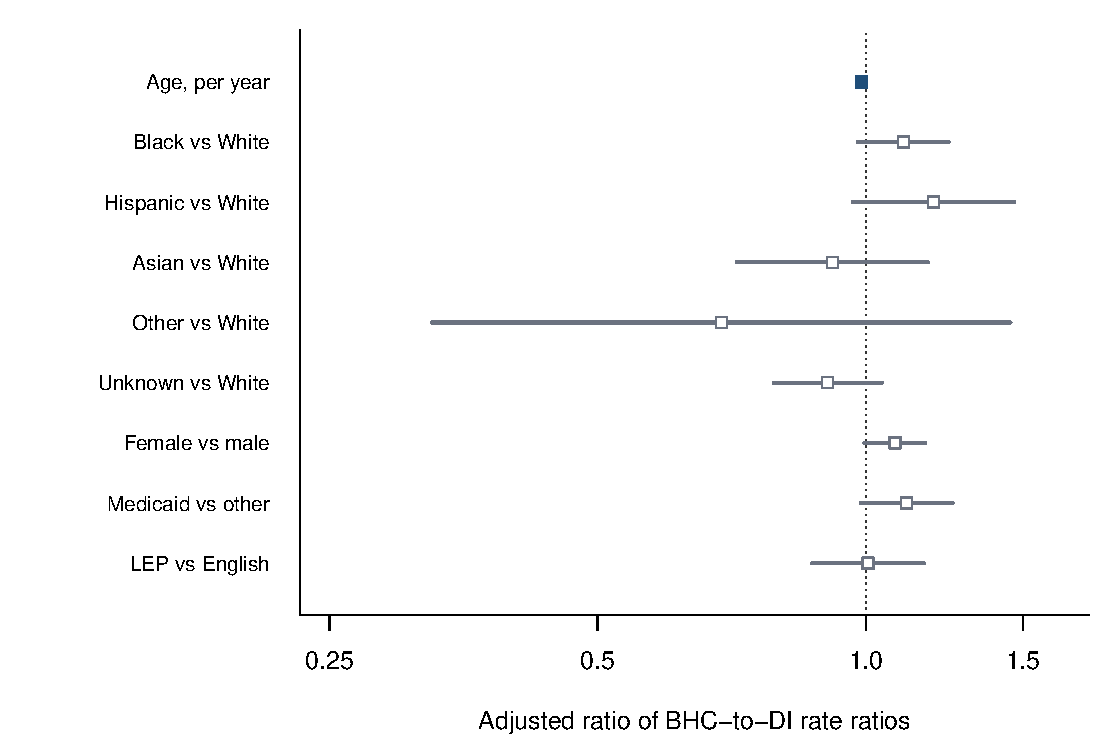
\includegraphics[width=0.82\linewidth]{figure3_identity.pdf}
\caption{Identity-related modification of the clinician-facing BHC to patient-facing DI rate ratio. Squares show adjusted interaction RRs and horizontal lines show 95\% CIs. Filled squares met the Benjamini-Hochberg false discovery threshold. BHC, Brief Hospital Course; DI, Discharge Instructions; LEP, limited English proficiency.}
\visiblealt{Forest plot with nine adjusted identity interaction estimates on a ratio scale. Age is the only filled marker and lies just below 1 with a narrow interval; the intervals for documented race and ethnicity, sex, Medicaid status, and limited English proficiency cross 1.}
\label{fig:s_identity}
\end{figure}

\subsection{Layer 2 disease-stratified identity results}

\begin{table}[H]
\caption{Primary Layer 2 fitted contrasts: full cohort, SUD, and SMI}
\label{tab:s_layer2a}
\centering
\small
\begin{tabular}{llrrrrr}
\toprule
Cohort & Contrast & Notes & Subjects & RR & 95\% CI & BH q \\
\midrule
ALL & Black vs White & 38,179 & 15,459 & 1.141 & 1.022-1.275 & 0.087 \\
ALL & Hispanic vs White & 13,532 & 6,202 & 1.245 & 1.018-1.522 & 0.098 \\
ALL & Asian vs White & 8,215 & 4,588 & 0.906 & 0.710-1.155 & 0.478 \\
ALL & Unknown vs White & 19,075 & 14,068 & 0.909 & 0.795-1.039 & 0.242 \\
ALL & Other vs White & 714 & 405 & 0.709 & 0.339-1.485 & 0.465 \\
ALL & Female vs male & 131,639 & 63,775 & 1.079 & 1.001-1.163 & 0.105 \\
ALL & Age per +1 year & 259,187 & 125,271 & 0.990 & 0.987-0.992 & \(1.76\times10^{-14}\) \\
ALL & Medicaid vs non-Medicaid & 41,485 & 21,257 & 1.105 & 0.987-1.237 & 0.150 \\
ALL & LEP vs English & 25,727 & 11,682 & 1.044 & 0.904-1.207 & 0.555 \\
SUD & Black vs White & 4,128 & 2,010 & 1.152 & 0.895-1.482 & 0.612 \\
SUD & Hispanic vs White & 1,516 & 837 & 1.043 & 0.757-1.436 & 0.924 \\
SUD & Asian vs White & 181 & 135 & 0.551 & 0.246-1.234 & 0.589 \\
SUD & Unknown vs White & 2,086 & 1,797 & 0.719 & 0.558-0.928 & 0.089 \\
SUD & Female vs male & 7,842 & 4,679 & 1.071 & 0.884-1.298 & 0.772 \\
SUD & Age per +1 year & 24,323 & 14,615 & 1.001 & 0.994-1.007 & 0.924 \\
SUD & Medicaid vs non-Medicaid & 8,774 & 5,104 & 0.912 & 0.765-1.088 & 0.612 \\
SUD & LEP vs English & 1,007 & 606 & 1.018 & 0.699-1.483 & 0.924 \\
SMI & Black vs White & 2,033 & 1,028 & 1.077 & 0.834-1.391 & 0.649 \\
SMI & Hispanic vs White & 560 & 308 & 1.217 & 0.730-2.031 & 0.602 \\
SMI & Asian vs White & 172 & 122 & 2.168 & 0.775-6.066 & 0.262 \\
SMI & Unknown vs White & 780 & 632 & 1.088 & 0.737-1.605 & 0.671 \\
SMI & Female vs male & 6,112 & 3,320 & 1.235 & 1.016-1.500 & 0.135 \\
SMI & Age per +1 year & 11,556 & 6,429 & 0.995 & 0.989-1.002 & 0.262 \\
SMI & Medicaid vs non-Medicaid & 3,216 & 1,951 & 1.306 & 1.042-1.637 & 0.135 \\
SMI & LEP vs English & 533 & 311 & 0.693 & 0.423-1.135 & 0.262 \\
\bottomrule
\end{tabular}
\end{table}

\begin{table}[H]
\caption{Primary Layer 2 fitted contrasts: chronic pain and obesity}
\label{tab:s_layer2b}
\centering
\small
\begin{tabular}{llrrrrr}
\toprule
Cohort & Contrast & Notes & Subjects & RR & 95\% CI & BH q \\
\midrule
Chronic pain & Black vs White & 2,668 & 1,338 & 0.999 & 0.690-1.447 & 0.996 \\
Chronic pain & Hispanic vs White & 813 & 483 & 1.128 & 0.585-2.176 & 0.996 \\
Chronic pain & Unknown vs White & 764 & 631 & 0.781 & 0.466-1.307 & 0.808 \\
Chronic pain & Female vs male & 8,171 & 4,703 & 1.208 & 0.916-1.592 & 0.808 \\
Chronic pain & Age per +1 year & 14,580 & 8,442 & 0.994 & 0.983-1.005 & 0.808 \\
Chronic pain & Medicaid vs non-Medicaid & 3,721 & 2,084 & 0.983 & 0.714-1.354 & 0.996 \\
Chronic pain & LEP vs English & 953 & 630 & 1.079 & 0.615-1.895 & 0.996 \\
Obesity & Black vs White & 5,947 & 3,101 & 0.982 & 0.683-1.413 & 0.969 \\
Obesity & Hispanic vs White & 1,560 & 968 & 1.474 & 0.558-3.890 & 0.882 \\
Obesity & Unknown vs White & 1,922 & 1,512 & 0.989 & 0.603-1.622 & 0.969 \\
Obesity & Female vs male & 16,009 & 9,238 & 1.371 & 1.013-1.855 & 0.286 \\
Obesity & Age per +1 year & 27,313 & 16,087 & 1.004 & 0.992-1.017 & 0.882 \\
Obesity & Medicaid vs non-Medicaid & 5,135 & 3,035 & 1.233 & 0.831-1.829 & 0.882 \\
Obesity & LEP vs English & 1,730 & 1,044 & 1.015 & 0.468-2.201 & 0.969 \\
\bottomrule
\end{tabular}
\end{table}

\begin{table}[H]
\caption{Primary Layer 2 fitted contrasts: HIV and ESRD}
\label{tab:s_layer2c}
\centering
\small
\begin{tabular}{llrrrrr}
\toprule
Cohort & Contrast & Notes & Subjects & RR & 95\% CI & BH q \\
\midrule
HIV & Black vs White & 1,454 & 448 & 0.573 & 0.288-1.140 & 0.263 \\
HIV & Hispanic vs White & 491 & 195 & 0.706 & 0.265-1.878 & 0.565 \\
HIV & Unknown vs White & 236 & 153 & 0.313 & 0.133-0.739 & 0.057 \\
HIV & Female vs male & 1,022 & 340 & 0.832 & 0.445-1.556 & 0.565 \\
HIV & Age per +1 year & 4,754 & 1,763 & 0.975 & 0.947-1.004 & 0.263 \\
HIV & Medicaid vs non-Medicaid & 1,578 & 633 & 1.247 & 0.670-2.321 & 0.565 \\
HIV & LEP vs English & 325 & 111 & 1.883 & 0.787-4.506 & 0.272 \\
ESRD & Black vs White & 3,475 & 784 & 1.169 & 0.805-1.698 & 0.688 \\
ESRD & Hispanic vs White & 822 & 208 & 1.189 & 0.511-2.767 & 0.688 \\
ESRD & Unknown vs White & 595 & 354 & 1.266 & 0.525-3.050 & 0.688 \\
ESRD & Female vs male & 3,911 & 1,132 & 0.894 & 0.610-1.309 & 0.688 \\
ESRD & Age per +1 year & 9,422 & 2,900 & 0.984 & 0.970-0.998 & 0.212 \\
ESRD & Medicaid vs non-Medicaid & 1,189 & 398 & 1.699 & 0.917-3.149 & 0.323 \\
ESRD & LEP vs English & 1,142 & 311 & 0.718 & 0.367-1.405 & 0.688 \\
\bottomrule
\end{tabular}
\end{table}

\begin{table}[H]
\caption{Primary Layer 2 fitted contrasts: diabetes}
\label{tab:s_layer2d}
\centering
\small
\begin{tabular}{llrrrrr}
\toprule
Cohort & Contrast & Notes & Subjects & RR & 95\% CI & BH q \\
\midrule
Diabetes & Black vs White & 15,102 & 5,055 & 1.270 & 1.045-1.544 & 0.056 \\
Diabetes & Hispanic vs White & 5,046 & 1,820 & 1.067 & 0.775-1.470 & 0.790 \\
Diabetes & Asian vs White & 2,263 & 1,064 & 0.833 & 0.533-1.301 & 0.690 \\
Diabetes & Unknown vs White & 5,012 & 3,435 & 0.890 & 0.666-1.189 & 0.690 \\
Diabetes & Female vs male & 33,152 & 13,475 & 0.981 & 0.845-1.138 & 0.796 \\
Diabetes & Age per +1 year & 71,103 & 29,229 & 0.988 & 0.982-0.994 & 0.001 \\
Diabetes & Medicaid vs non-Medicaid & 10,794 & 4,708 & 1.339 & 1.045-1.716 & 0.056 \\
Diabetes & LEP vs English & 9,868 & 3,955 & 0.930 & 0.727-1.189 & 0.750 \\
\bottomrule
\end{tabular}
\end{table}

Only age within diabetes reached \(q<0.05\) among disease-stratified contrasts. The ALL rows are a replication under the Layer 2 formula and should not replace the jointly adjusted Layer 1 estimates.

\clearpage
\begin{table}[H]
\centering
\caption{Layer 2 dropped-cell audit}
\label{tab:s_layer2_drop}
\resizebox{\linewidth}{!}{%
\begin{tabular}{lllrrrr}
\toprule
Cohort & Axis or level & Reason & Notes & Subjects & BHC events & DI events \\
\midrule
SUD & race=Other & Event floor & 102 & 68 & 40 & 3 \\
SMI & race=Other & Event floor & 27 & 21 & 18 & 3 \\
Sickle cell disease & all identity contrasts & Cohort notes below 1,000 & 419 & 131 & NA & NA \\
Chronic pain & race=Asian & Event floor & 145 & 109 & 39 & 2 \\
Chronic pain & race=Other & Event floor & 26 & 21 & 11 & 0 \\
Obesity & race=Asian & Event floor & 185 & 125 & 40 & 1 \\
Obesity & race=Other & Event floor & 105 & 64 & 24 & 0 \\
HIV & race=Asian & Event floor & 37 & 18 & 23 & 0 \\
HIV & race=Other & Event floor & 18 & 6 & 0 & 0 \\
ESRD & race=Asian & Event floor & 370 & 127 & 74 & 2 \\
ESRD & race=Other & Event floor & 71 & 31 & 11 & 1 \\
Diabetes & race=Other & Event floor & 215 & 104 & 51 & 2 \\
\bottomrule
\end{tabular}}
\end{table}

\subsection{Layer 3 primary disease results}

\begin{table}[H]
\caption{Primary Layer 3 disease modification estimates}
\label{tab:s_layer3}
\resizebox{\linewidth}{!}{%
\begin{tabular}{lrrrrrrrl}
\toprule
Contrast & Notes & Subjects & BHC/1k & DI/1k & RR & 95\% CI & \(p\) & BH q \\
\midrule
Diabetes & 71,318 & 29,315 & 0.657 & 0.067 & 1.275 & 1.155-1.408 & \(1.57\times10^{-6}\) & \(1.26\times10^{-5}\) \\
SMI & 11,583 & 6,444 & 1.872 & 0.237 & 0.725 & 0.632-0.832 & \(4.88\times10^{-6}\) & \(1.95\times10^{-5}\) \\
Obesity & 27,603 & 16,265 & 0.598 & 0.040 & 1.376 & 1.189-1.592 & \(1.83\times10^{-5}\) & \(4.87\times10^{-5}\) \\
Sickle cell disease & 419 & 131 & 1.180 & 0.261 & 0.392 & 0.188-0.817 & 0.013 & 0.025 \\
HIV & 4,809 & 1,785 & 1.120 & 0.097 & 1.470 & 1.053-2.053 & 0.024 & 0.038 \\
SUD & 24,425 & 14,678 & 1.340 & 0.158 & 0.910 & 0.808-1.025 & 0.121 & 0.161 \\
ESRD & 9,863 & 3,049 & 0.680 & 0.084 & 0.936 & 0.770-1.139 & 0.509 & 0.582 \\
Chronic pain & 14,751 & 8,569 & 0.887 & 0.105 & 0.986 & 0.828-1.175 & 0.876 & 0.876 \\
\bottomrule
\end{tabular}}
\end{table}

\begin{table}[H]
\caption{Scored candidates and stigmatizing-language events by anchor family and section}
\label{tab:s_families}
\centering
\small
\begin{tabular}{llrrrr}
\toprule
Section & Anchor family & Scored candidates & Stigma events & $P$(stigma$\mid$scored) & Share of section events \\
\midrule
BHC & Credibility/obstinance & 3,321 & 3,212 & 0.967 & 5.0\% \\
BHC & Compliance & 55,300 & 41,183 & 0.745 & 64.3\% \\
BHC & Other & 41,854 & 19,614 & 0.469 & 30.6\% \\
HPI & Credibility/obstinance & 2,310 & 2,117 & 0.916 & 7.3\% \\
HPI & Compliance & 20,361 & 13,803 & 0.678 & 47.3\% \\
HPI & Other & 22,858 & 13,276 & 0.581 & 45.5\% \\
DI & Credibility/obstinance & 145 & 136 & 0.938 & 3.8\% \\
DI & Compliance & 5,766 & 2,156 & 0.374 & 60.5\% \\
DI & Other & 2,702 & 1,273 & 0.471 & 35.7\% \\
\bottomrule
\end{tabular}
\begin{tablenotes}
\item Probabilities use successfully relocated and scored candidates. The 89 relocation failures comprised 72 BHC-other, 12 HPI-other, 1 HPI-compliance, and 4 DI-other candidates and are excluded from these denominators. Event shares sometimes differ slightly from 100\% because of rounding. BHC, Brief Hospital Course; HPI, History of Present Illness; DI, Discharge Instructions.
\end{tablenotes}
\end{table}

\begin{table}[H]
\caption{Direct standardization of conditional stigma probabilities to a pooled anchor-family distribution}
\label{tab:s_family_standardization}
\centering
\small
\begin{tabular}{lrrrrrrr}
\toprule
Comparison & Crude $P_A$ & Crude $P_{DI}$ & Crude ratio & Standardized $P_A$ & Standardized $P_{DI}$ & Standardized ratio & Composition share \\
\midrule
BHC vs DI & 0.637 & 0.414 & 1.54 & 0.639 & 0.432 & 1.48 & $-1.3\%$ \\
HPI vs DI & 0.641 & 0.414 & 1.55 & 0.643 & 0.445 & 1.44 & 6.0\% \\
\bottomrule
\end{tabular}
\begin{tablenotes}
\item Standardized probabilities apply the candidate-count distribution pooled across the two sections to each section's three family-specific probabilities. Composition share is the symmetric Kitagawa composition component divided by the crude conditional-probability difference; a negative value indicates that broad-family composition slightly masked the difference. The complementary within-family shares were 101.3\% for BHC-DI and 94.0\% for HPI-DI. BHC, Brief Hospital Course; HPI, History of Present Illness; DI, Discharge Instructions.
\end{tablenotes}
\end{table}

\begin{table}[H]
\caption{Distribution of within-note section token shares}
\label{tab:s_section_shares}
\centering
\small
\begin{tabular}{lrrrr}
\toprule
Token-share metric & Notes & Mean (SD), \% & Median (IQR), \% & 5th--95th percentile, \% \\
\midrule
BHC share of BHC+DI & 259,207 & 63.0 (18.8) & 67.6 (51.3--77.5) & 26.1--86.7 \\
HPI share of HPI+DI & 252,581 & 52.3 (23.3) & 58.2 (34.9--70.9) & 8.2--82.4 \\
BHC share of BHC+HPI+DI & 252,581 & 44.0 (14.2) & 44.2 (33.9--53.9) & 20.1--67.3 \\
HPI share of BHC+HPI+DI & 252,581 & 28.5 (14.5) & 28.3 (17.5--38.3) & 5.2--53.0 \\
DI share of BHC+HPI+DI & 252,581 & 27.5 (17.8) & 21.2 (14.5--36.0) & 8.7--65.9 \\
\bottomrule
\end{tabular}
\begin{tablenotes}
\item Shares were calculated within each note before summarization. BHC, Brief Hospital Course; HPI, History of Present Illness; DI, Discharge Instructions; SD, standard deviation; IQR, interquartile range.
\end{tablenotes}
\end{table}

\begin{table}[H]
\caption{Crude age-stratified absolute section rates and BHC-DI contrasts}
\label{tab:s_age_rates}
\centering
\small
\resizebox{\linewidth}{!}{%
\begin{tabular}{lrrrrrr}
\toprule
Age, years & Notes & BHC events & BHC/1,000 (95\% CI) & DI events & DI/1,000 (95\% CI) & Crude RR (95\% CI) \\
\midrule
18--39 & 33,680 & 10,919 & 0.936 (0.918--0.954) & 486 & 0.068 (0.062--0.074) & 13.83 (12.63--15.15) \\
40--64 & 103,057 & 25,560 & 0.673 (0.665--0.682) & 1,287 & 0.056 (0.053--0.060) & 11.94 (11.29--12.62) \\
65--79 & 75,296 & 15,221 & 0.506 (0.498--0.515) & 878 & 0.052 (0.049--0.056) & 9.74 (9.10--10.42) \\
80 or older & 47,154 & 12,306 & 0.608 (0.597--0.619) & 914 & 0.099 (0.093--0.106) & 6.14 (5.75--6.57) \\
\bottomrule
\end{tabular}}
\begin{tablenotes}
\item Rates are crude events per 1,000 section tokens in the 259,187-note complete-case cohort. Rate intervals are exact Poisson intervals; crude RR intervals use the log-event approximation. BHC, Brief Hospital Course; DI, Discharge Instructions; RR, rate ratio.
\end{tablenotes}
\end{table}

\begin{figure}[H]
\centering
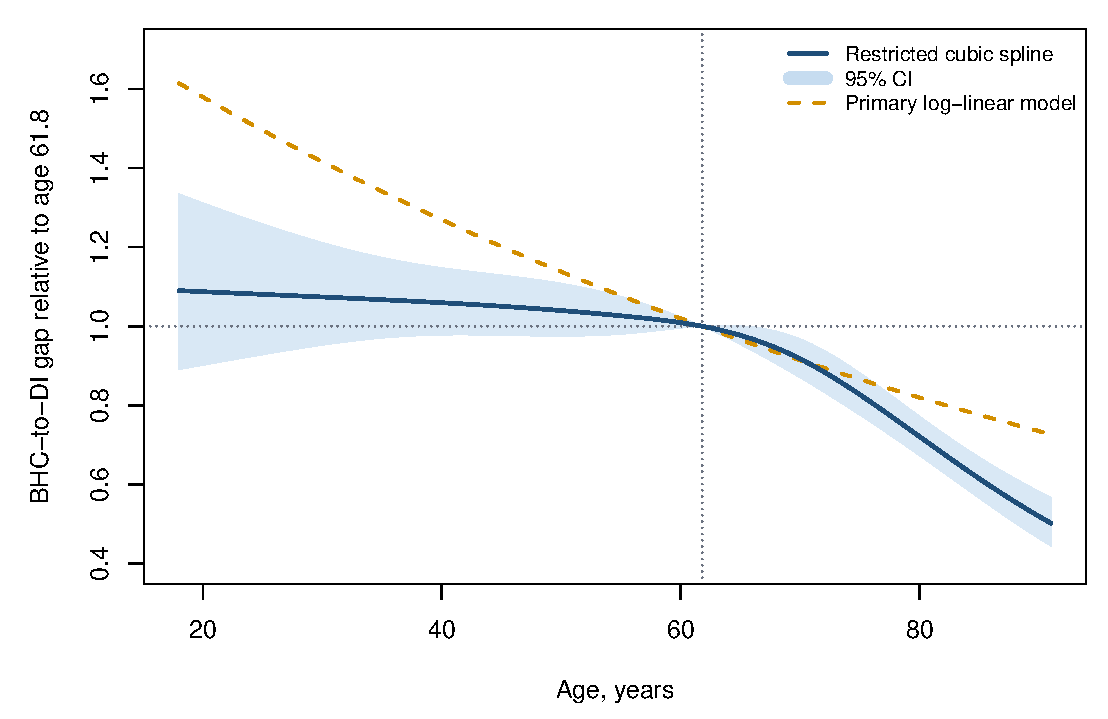
\includegraphics[width=0.82\linewidth]{figure_s2_age_nonlinearity.pdf}
\caption{Nonlinear age diagnostic for the adjusted clinician-facing BHC to patient-facing DI gap. The solid line and band show the restricted cubic spline estimate and 95\% CI relative to the fitted gap at the sample mean age of 61.8 years. The dashed line shows the primary log-linear age specification. Spline knots were 28, 56, 70, and 89 years. The joint robust Wald test for the two nonlinear interaction terms was $\chi^2_2=42.16$ ($P=6.99\times10^{-10}$). BHC, Brief Hospital Course; DI, Discharge Instructions.}
\visiblealt{Line plot from age 18 to 91. The restricted cubic spline curve stays near 1 through middle age and then falls, reaching about 0.72 at age 80 and 0.52 at age 90 relative to age 61.8. The primary log-linear line declines steadily and differs most at younger and older ages.}
\label{fig:s_age_nonlinearity}
\end{figure}

\subsection{LLM verification of disease cohorts}

Votes were strongly polarized (Table~\ref{tab:s_llm_votes}). All five models labeled 124,308 admission--disease pairs (75.44\%) as SUPPORTED, and none did for 23,834 pairs (14.47\%); together these unanimous outcomes covered 89.91\% of pairs. Only 8,499 pairs (5.16\%) received two or three SUPPORTED votes, so the choice of vote threshold affects a small share of the cohort. All five models assigned the same three-class label to 146,100 pairs (88.67\%).

Overall agreement was almost perfect by Landis and Koch benchmarks (Table~\ref{tab:s_llm_overall}): Fleiss \(\kappa\) was 0.816 for three classes and 0.838 for the binary outcome, and Krippendorff \(\alpha\) was 0.817 and 0.839. Because \(\alpha\) accommodates missing ratings and differed from \(\kappa\) by less than 0.001, the 651 unparsed outputs did not materially affect agreement. Binary pairwise \(\kappa\) ranged from 0.770 to 0.913, with a median of 0.841, and all 10 pairs exceeded 0.60 (Table~\ref{tab:s_llm_pairwise}).

Models differed in how readily they assigned SUPPORTED (Table~\ref{tab:s_llm_models}). GLM-4-32B was the most permissive (83.89\%) and had the lowest mean pairwise \(\kappa\) (0.814); Qwen3.5-27B was the most conservative (77.97\%), a difference of 5.9 percentage points. REFUTED was rarely assigned by any model (0.13\%--1.68\%). The procedure therefore separates notes that document a coded condition from notes that do not provide evidence for it; it should not be used to conclude that a patient does not have the condition.

Support rates varied by disease (Table~\ref{tab:s_llm_disease}). The share of pairs with at least three SUPPORTED votes ranged from 58.2\% for chronic pain to 96.5\% for HIV. Agreement and support rates were not aligned. HIV had the highest support rate but the lowest \(\kappa\) (0.614), because when nearly all labels are SUPPORTED, expected chance agreement is high and \(\kappa\) is reduced. Obesity had a lower support rate (68.1\%) but the highest \(\kappa\) (0.895), indicating that the models agreed on which obesity codes lacked documentary support. A low \(\kappa\) should therefore be read alongside the support rate rather than as evidence of unreliable adjudication.

Support declined with the position of the qualifying code in the diagnosis sequence (Table~\ref{tab:s_llm_icd}). At least three models supported 94.1\% of principal-diagnosis pairs, 83.9\% of middle-position pairs, and 72.0\% of late-position pairs, and the share with no SUPPORTED votes rose from 2.4\% to 11.8\% and 22.2\%. Principal diagnoses accounted for only 5.7\% of adjudicated pairs, so most disease-cohort membership rested on secondary codes.

Restricting disease cohorts to LLM-verified pairs left the main disease findings unchanged in direction (Table~\ref{tab:s_llm_layer3}). Obesity and diabetes continued to widen the adjusted BHC-DI gap, and serious mental illness and sickle cell disease continued to narrow it, under both vote thresholds. Two cohorts changed in their false discovery classification. Substance use disorder, which was not significant in the ICD-coded cohort (RR, 0.910), showed a narrower gap after verification (RR, 0.825 at three or more votes and 0.829 at five votes). The HIV estimate attenuated from 1.470 to 1.396 at five votes and no longer met the false discovery threshold. End-stage renal disease and chronic pain remained null at both thresholds.

\begin{table}[H]
\caption{Distribution of SUPPORTED votes across five LLMs per admission--disease pair}
\label{tab:s_llm_votes}
\centering
\small
\begin{tabular}{lrrr}
\toprule
SUPPORTED votes & Pairs & Share (\%) & Cumulative (\%) \\
\midrule
0/5 & 23,834 & 14.47 & 14.47 \\
1/5 & 3,717 & 2.26 & 16.72 \\
2/5 & 4,034 & 2.45 & 19.17 \\
3/5 & 4,465 & 2.71 & 21.88 \\
4/5 & 4,412 & 2.68 & 24.56 \\
5/5 & 124,308 & 75.44 & 100.00 \\
\midrule
Total & 164,770 & 100.00 & \\
\bottomrule
\end{tabular}
\begin{tablenotes}
\item The adjudication covered 164,770 admission--disease pairs from 122,301 admissions and eight disease cohorts, with 823,850 model inferences. Unparsed outputs (651) were treated as missing votes. LLM, large language model.
\end{tablenotes}
\end{table}

\begin{table}[H]
\caption{Overall agreement among five LLMs}
\label{tab:s_llm_overall}
\centering
\small
\begin{tabular}{lrr}
\toprule
Metric & Three classes & Binary \\
\midrule
Fleiss \(\kappa\) & 0.8159 & 0.8383 \\
Krippendorff \(\alpha\) & 0.8167 & 0.8391 \\
Complete agreement (\%) & 88.67 & 89.91 \\
\bottomrule
\end{tabular}
\begin{tablenotes}
\item Three classes are SUPPORTED, REFUTED, and INSUFFICIENT. The binary outcome is SUPPORTED versus REFUTED or INSUFFICIENT. Complete agreement is the share of pairs on which all five models assigned the same label.
\end{tablenotes}
\end{table}

\begin{table}[H]
\caption{Pairwise agreement between LLMs}
\label{tab:s_llm_pairwise}
\centering
\small
\begin{tabular}{llrrrr}
\toprule
Model A & Model B & 3-class agr. (\%) & 3-class \(\kappa\) & Binary agr. (\%) & Binary \(\kappa\) \\
\midrule
Qwen3.5-27B & Gemma-4-31B & 96.3 & 0.894 & 97.0 & 0.913 \\
GLM-4-32B & Mistral-24B & 95.4 & 0.836 & 96.6 & 0.876 \\
gpt-oss-20b & Gemma-4-31B & 95.0 & 0.848 & 95.8 & 0.871 \\
Qwen3.5-27B & gpt-oss-20b & 95.3 & 0.858 & 95.6 & 0.867 \\
Mistral-24B & gpt-oss-20b & 95.4 & 0.846 & 95.6 & 0.852 \\
Qwen3.5-27B & Mistral-24B & 94.2 & 0.818 & 94.6 & 0.830 \\
GLM-4-32B & gpt-oss-20b & 93.9 & 0.792 & 95.0 & 0.828 \\
Mistral-24B & Gemma-4-31B & 93.0 & 0.779 & 93.8 & 0.804 \\
Qwen3.5-27B & GLM-4-32B & 92.1 & 0.749 & 93.2 & 0.781 \\
GLM-4-32B & Gemma-4-31B & 92.1 & 0.748 & 92.9 & 0.770 \\
\bottomrule
\end{tabular}
\begin{tablenotes}
\item Rows are ordered by binary \(\kappa\). Agr., observed agreement.
\end{tablenotes}
\end{table}

\begin{table}[H]
\caption{Label distribution by LLM}
\label{tab:s_llm_models}
\centering
\small
\begin{tabular}{lrrrr}
\toprule
Model & SUPPORTED (\%) & REFUTED (\%) & INSUFFICIENT (\%) & Mean pairwise \(\kappa\) \\
\midrule
GLM-4-32B & 83.89 & 1.68 & 14.38 & 0.814 \\
Mistral-24B & 82.65 & 0.29 & 17.05 & 0.841 \\
gpt-oss-20b & 80.46 & 0.13 & 19.06 & 0.855 \\
Gemma-4-31B & 78.23 & 1.08 & 20.69 & 0.839 \\
Qwen3.5-27B & 77.97 & 0.53 & 21.50 & 0.847 \\
\bottomrule
\end{tabular}
\begin{tablenotes}
\item Percentages use all 164,770 pairs as the denominator; rows do not sum to 100\% where outputs could not be parsed. Mean pairwise \(\kappa\) averages the binary \(\kappa\) of each model with the other four.
\end{tablenotes}
\end{table}

\begin{table}[H]
\caption{LLM agreement and support by disease cohort}
\label{tab:s_llm_disease}
\centering
\small
\begin{tabular}{lrrrrrrr}
\toprule
Disease cohort & Pairs & Fleiss \(\kappa\) & Complete agr. (\%) & 5/5 (\%) & \(\geq\)3/5 (\%) & \(\geq\)1/5 (\%) & 0/5 (\%) \\
\midrule
HIV & 4,809 & 0.614 & 95.0 & 93.9 & 96.5 & 98.9 & 1.1 \\
Sickle cell disease & 419 & 0.860 & 93.1 & 90.0 & 93.1 & 94.3 & 5.7 \\
Diabetes & 71,317 & 0.744 & 93.3 & 89.6 & 92.8 & 95.9 & 4.1 \\
End-stage renal disease & 9,863 & 0.702 & 85.6 & 84.8 & 91.0 & 95.4 & 4.6 \\
Serious mental illness & 11,583 & 0.815 & 83.6 & 75.0 & 79.4 & 86.8 & 13.2 \\
Obesity & 27,603 & 0.895 & 89.3 & 61.0 & 68.1 & 71.1 & 28.9 \\
Substance use disorder & 24,425 & 0.805 & 80.7 & 57.6 & 67.4 & 74.9 & 25.1 \\
Chronic pain & 14,751 & 0.840 & 82.1 & 51.3 & 58.2 & 67.8 & 32.2 \\
\bottomrule
\end{tabular}
\begin{tablenotes}
\item Fleiss \(\kappa\) and complete agreement use the three labels. Vote columns give the share of pairs with the stated number of SUPPORTED votes out of five. Agr., agreement.
\end{tablenotes}
\end{table}

\begin{table}[H]
\caption{LLM agreement and support by position of the qualifying ICD code}
\label{tab:s_llm_icd}
\centering
\small
\begin{tabular}{lrrrrrr}
\toprule
Code position & Pairs & Share (\%) & Fleiss \(\kappa\) & 5/5 (\%) & \(\geq\)3/5 (\%) & 0/5 (\%) \\
\midrule
Principal (sequence 1) & 9,380 & 5.7 & 0.644 & 89.8 & 94.1 & 2.4 \\
Middle (sequence 2--9) & 105,152 & 63.8 & 0.828 & 78.8 & 83.9 & 11.8 \\
Late (sequence \(\geq\)10) & 50,238 & 30.5 & 0.853 & 65.7 & 72.0 & 22.2 \\
\bottomrule
\end{tabular}
\begin{tablenotes}
\item Position is the sequence number of the qualifying diagnosis code within the admission. Vote columns give the share of pairs with the stated number of SUPPORTED votes out of five.
\end{tablenotes}
\end{table}

\begin{table}[H]
\caption{Layer 3 disease interaction RRs in ICD-coded and LLM-verified disease cohorts}
\label{tab:s_llm_layer3}
\centering
\small
\begin{tabular}{llll}
\toprule
Disease cohort & ICD-coded & \(\geq\)3/5 SUPPORTED votes & 5/5 SUPPORTED votes \\
\midrule
Serious mental illness & 0.725 (0.63-0.83)*** & 0.740 (0.64-0.86)*** & 0.753 (0.65-0.88)** \\
Sickle cell disease & 0.392 (0.19-0.82)* & 0.323 (0.17-0.60)*** & 0.359 (0.16-0.79)* \\
Substance use disorder & 0.910 (0.81-1.03) & 0.825 (0.72-0.95)** & 0.829 (0.72-0.96)* \\
Chronic pain & 0.986 (0.83-1.18) & 0.992 & 1.010 \\
HIV & 1.470 (1.05-2.05)* & 1.399 (1.01-1.94) & 1.396 (1.00-1.96) \\
End-stage renal disease & 0.936 (0.77-1.14) & 0.882 & 0.848 \\
Diabetes & 1.275 (1.15-1.41)*** & 1.308 (1.18-1.44)*** & 1.291 (1.17-1.43)*** \\
Obesity & 1.376 (1.19-1.59)*** & 1.347 (1.13-1.61)** & 1.329 (1.11-1.60)** \\
\bottomrule
\end{tabular}
\begin{tablenotes}
\item Values are covariate-adjusted interaction RRs (95\% CI) comparing the BHC-DI rate ratio for notes with versus without each condition. The ICD-coded column reproduces the primary Layer 3 estimates (Table~\ref{tab:s_layer3}). Verified columns restrict each disease cohort to admission--disease pairs with the stated number of SUPPORTED votes from five LLMs. Asterisks mark Benjamini-Hochberg \(q<0.05\) (*), \(q<0.01\) (**), and \(q<0.001\) (***); unmarked estimates did not meet \(q<0.05\). BHC, Brief Hospital Course; DI, Discharge Instructions; LLM, large language model.
\end{tablenotes}
\end{table}
% TODO(HY): add 95% CIs for chronic pain and end-stage renal disease in the two verified columns.

\section{Supplementary Note: Data Processing and Variable Definitions}
\label{sec:s_processing}

This note documents each processing step between the source data and the analysis dataset, together with the code lists used to define disease cohorts and comorbidity. Counts refer to the primary sentence-window analysis.

\subsection{Source data}

Discharge summaries came from the discharge file of MIMIC-IV-Note version 2.2, read with Latin-1 encoding. Patient, admission, and diagnosis tables came from the hosp module of MIMIC-IV version 3.1. % TODO(HY): the main text and reference list cite MIMIC-IV version 2.2; confirm which version was used and align all three.
The stigmatizing-language resource of Harrigian and colleagues (version 1.0.0) supplied the 89-term keyword lexicon and the 5,043 annotated training instances.

\subsection{Section segmentation and cohort construction}

Each discharge summary was divided into sections using regular expressions for 25 fixed section headers. A header was recognized only at the start of a line and when followed by a colon; matching ignored case, and longer headers were matched before shorter ones. Subheadings within the physical examination, such as HEENT, were deliberately not treated as section boundaries. When a header occurred more than once in a note, only the first occurrence was kept. A token was defined as a maximal run of word characters (letters, digits, or underscore), and section length was the number of such tokens.

A note entered the section-analysis cohort if it contained both a BHC and a DI section with at least 50 tokens each (Table~\ref{tab:s_flow}). The Follow-up Instructions section is replaced by an empty string during deidentification in MIMIC-IV-Note and was therefore excluded. The Social History section averaged about three tokens per note and was not used in the primary models.

\begin{table}[H]
\caption{Construction of the analysis cohorts}
\label{tab:s_flow}
\centering
\small
\begin{tabular}{lr}
\toprule
Step & Notes \\
\midrule
Discharge summaries scanned & 331,793 \\
\quad Excluded: BHC or DI section absent & 41,788 \\
Notes with both BHC and DI & 290,005 \\
\quad Excluded: BHC or DI shorter than 50 tokens & 30,798 \\
Section-analysis cohort & 259,207 \\
\quad Excluded: no linked patient or admission record & 20 \\
Group-analysis cohort (complete cases) & 259,187 \\
\bottomrule
\end{tabular}
\begin{tablenotes}
\item Each note corresponds to one hospital admission. The group-analysis cohort contained 125,271 patients. BHC, Brief Hospital Course; DI, Discharge Instructions.
\end{tablenotes}
\end{table}

\subsection{Keyword candidates and scoring}

The 89 lexicon terms fall into three non-overlapping families: 13 adamant terms, 26 compliance terms, and 50 other terms. Keyword matching ignored case and required that the match not be preceded or followed by a letter, digit, or underscore. A space within a multiword term could match either a space or a hyphen, so that drug seeking also matched drug-seeking, and longer terms were matched before shorter ones. Because a hyphen counts as a boundary under this rule, non-compliance was matched as the term compliance rather than as noncompliance; whether such a match was stigmatizing was left to the classifier.

For scoring, each candidate was represented by the sentence containing the keyword and one sentence on either side, taken from the original section text. Sentence boundaries were a period, question mark, or exclamation mark followed by whitespace. The window was then cleaned and normalized with the procedures released with the annotation resource, and the keyword was located again in the normalized text. When the keyword occurred more than once in the window, the occurrence nearest the window midpoint was marked. Inputs longer than 256 tokens were truncated, and each candidate received the label with the higher predicted score. Candidates whose keyword could not be found after normalization were excluded from event counts (Table~\ref{tab:s_candidates}). When the same keyword occurred twice within one three-sentence window, both candidates were marked at the same occurrence, so one of the two was anchored to the wrong position.

\begin{table}[H]
\caption{Keyword candidates, relocation failures, and scored candidates by section}
\label{tab:s_candidates}
\centering
\small
\begin{tabular}{lrrr}
\toprule
Section & Candidates & Relocation failures & Scored \\
\midrule
BHC & 100,547 & 72 & 100,475 \\
HPI & 45,542 & 13 & 45,529 \\
DI & 8,617 & 4 & 8,613 \\
Social History & 278 & 0 & 278 \\
\midrule
Total & 154,984 & 89 & 154,895 \\
\bottomrule
\end{tabular}
\begin{tablenotes}
\item Social History candidates were scored but not used in the primary models. BHC, Brief Hospital Course; HPI, History of Present Illness; DI, Discharge Instructions.
\end{tablenotes}
\end{table}

\subsection{Classifier training data}

The coordinates of the 5,043 annotations are defined on text processed with the cleaning and normalization procedures released with the resource. After applying the same procedures, every annotated keyword was located (5,043 of 5,043). Each training input contained the keyword sentence and one sentence on either side, with the keyword enclosed by the reserved tokens [unused1] and [unused2]. Negative, disbelief, and difficult annotations formed the stigma class; neutral, positive, and exclude annotations formed the non-stigma class. Instances were split 80/10/10 by note identifier with a fixed random seed of 42, giving 4,037 training, 501 validation, and 505 test instances.

Two features of the training data bear on interpretation. First, the split was made by note rather than by patient, so different notes from the same patient could fall in the training and test sets. Second, 3,552 of the 4,710 annotated notes were also in the 259,207-note analysis cohort, about 1.4\% of the cohort, so the classifier scored some passages it had seen during training.
% TODO(HY): consider a sensitivity analysis excluding these 3,552 notes, or add this point to the main-text limitations.

\subsection{Analysis dataset}

The analysis dataset contained one row for each BHC, HPI, and DI section of each cohort note: 259,207 BHC rows, 259,207 DI rows, and 252,581 HPI rows, for 770,995 rows in total. Notes without an HPI section had no HPI row. Stigmatizing-language events were counted for each note and section and merged onto these rows, and sections with no events were kept with a count of zero (713,965 rows).

Every note was linked to its patient and admission identifiers without loss. Twenty notes (57 rows) had no matching patient or admission record and therefore lacked sex and age; these were removed in the final complete-case step. The remaining covariates were coded as follows.

Medicaid status was 1 when the recorded insurance was Medicaid and 0 for Medicare, private, other, no charge, or missing insurance (missing for 2,793 notes). Limited English proficiency was 1 for any recorded language other than English, including the category Other (677 admissions), and missing language was coded as English (398 notes). Age was the anchor age plus the difference between the admission year and the anchor year, truncated to 18--91 years and centered at the sample mean. Length of stay was discharge time minus admission time, with negative values set to zero, and entered the models as \(\log(1+\text{days})\).

Race and ethnicity were assigned from the recorded category by checking, in order, for Black, Hispanic or Latino, Asian, White, and American Indian or Alaska Native or Native Hawaiian or Pacific Islander; all remaining values were coded as Unknown. The Unknown group (19,075 admissions) comprised Other (8,709), Unknown (6,816), Patient Declined (1,082), Portuguese (989), Unable to Obtain (922), South American (302), and Multiple Race (255). The Other group (714 admissions) comprised American Indian or Alaska Native (503) and Native Hawaiian or Pacific Islander (211).
% TODO(HY): decide whether South American should be coded as Hispanic or Latino and how Portuguese should be coded.

For modeling, BHC was coded 1 and DI 0, and the offset was the log of the section token count with a floor of one token. The complete-case step on race and ethnicity, sex, Medicaid status, limited English proficiency, age, and token count removed 57 rows from 20 notes, all of them the unlinked notes above. The final group-analysis dataset contained 259,187 notes (one per admission) from 125,271 patients, with 518,374 BHC and DI rows, of which 481,383 had zero events, and 770,938 rows across all three sections.

\subsection{Disease cohort definitions}

Disease indicators were derived from all diagnosis codes recorded for each admission (Table~\ref{tab:s_disease_codes}). MIMIC-IV stores codes without decimal points; codes were stripped of surrounding whitespace and converted to upper case before matching. Code lists were applied separately by ICD version, so ICD-9 prefixes were matched only against ICD-9 codes and ICD-10 prefixes only against ICD-10 codes. A code was positive when it began with an inclusion prefix and did not begin with an exclusion prefix. An admission was assigned a condition when any of its codes was positive, regardless of the code's position in the diagnosis sequence; admissions had up to 57 codes. Ninety-one admissions had no recorded diagnosis codes and were coded as having none of the eight conditions and a Charlson score of zero.
% TODO(HY): pending code-list corrections: (1) remove ICD-9 282.64 from the sickle cell exclusions (it is sickle-cell/Hb-C disease with crisis; trait is 282.5, which is outside 282.6); (2) decide whether obesity should include overweight (278.02, E66.3; 354 admissions qualify only through these codes); (3) remove 296.82 and 298.0 from SMI (13 admissions); (4) add ICD-9 291 and 292 to SUD to match the scope of ICD-10 F10--F19 (966 admissions); (5) decide how to code the 91 admissions without diagnosis codes. Update this section and Table S25 after re-running.

\begin{table}[H]
\caption{ICD code definitions of the eight disease cohorts}
\label{tab:s_disease_codes}
\centering
\footnotesize
\setlength{\tabcolsep}{3pt}
\begin{tabular}{@{}>{\raggedright\arraybackslash}p{0.13\linewidth}>{\raggedright\arraybackslash}p{0.25\linewidth}>{\raggedright\arraybackslash}p{0.22\linewidth}>{\raggedright\arraybackslash}p{0.22\linewidth}r@{}}
\toprule
Cohort & ICD-9 inclusion & ICD-10 inclusion & Exclusion & Notes / patients \\
\midrule
Substance use disorder & 303 alcohol dependence; 304 drug dependence; 305 nondependent abuse & F10--F16, F18, F19 & 305.1 and F17 (tobacco) & 24,425 / 14,678 \\
Serious mental illness & 295 schizophrenic disorders; 296.0, 296.1, 296.4--296.8 bipolar disorders; 297 delusional disorders; 298 other nonorganic psychoses & F20--F25, F28, F29 psychotic disorders; F30 manic episode; F31 bipolar disorder & None; major depressive disorder (296.2, 296.3, F32, F33) not included & 11,583 / 6,444 \\
Sickle cell disease & 282.6 & D57 & 282.64; D57.3 (sickle cell trait) & 419 / 131 \\
Chronic pain & 338.2 chronic pain; 338.4 chronic pain syndrome & G89.2, G89.4 & None; neoplasm-related pain (338.3, G89.3) not included & 14,751 / 8,569 \\
Obesity & 278.0 & E66 & None & 27,603 / 16,265 \\
HIV & 042 symptomatic HIV disease; V08 asymptomatic HIV infection status & B20, Z21 & None & 4,809 / 1,785 \\
End-stage renal disease & 585.6 & N18.6 & None; chronic kidney disease stages 1--5 not included & 9,863 / 3,049 \\
Diabetes & 250 & E08 underlying condition; E09 drug induced; E10 type 1; E11 type 2; E13 other & None; gestational diabetes (O24) and prediabetes (R73) not included & 71,318 / 29,315 \\
\bottomrule
\end{tabular}
\begin{tablenotes}
\item Codes are shown with decimal points, and each entry matches every code that begins with it. ICD-9 278.0 includes 278.02 (overweight) and ICD-10 E66 includes E66.3 (overweight). ICD-9 alcohol-induced (291) and drug-induced (292) mental disorders were not included in substance use disorder. Notes and patients are counted in the group-analysis cohort.
\end{tablenotes}
\end{table}

\subsection{Charlson Comorbidity Index}

Severity was summarized with the Charlson Comorbidity Index, computed once per admission from all diagnosis codes, using the coding algorithm of Quan and colleagues and the original Charlson weights (Table~\ref{tab:s_charlson}). When both levels of a condition were present, only the more severe level was counted: moderate or severe liver disease superseded mild liver disease, metastatic solid tumor superseded any malignancy, and diabetes with complications superseded diabetes without complications.

\begin{table}[H]
\caption{Charlson Comorbidity Index conditions, weights, and ICD code prefixes}
\label{tab:s_charlson}
\centering
\scriptsize
\setlength{\tabcolsep}{3pt}
\begin{tabular}{@{}>{\raggedright\arraybackslash}p{0.15\linewidth}c>{\raggedright\arraybackslash}p{0.36\linewidth}>{\raggedright\arraybackslash}p{0.40\linewidth}@{}}
\toprule
Condition & Weight & ICD-9 & ICD-10 \\
\midrule
Myocardial infarction & 1 & 410, 412 & I21, I22, I25.2 \\
Congestive heart failure & 1 & 398.91, 402.01, 402.11, 402.91, 404.01, 404.03, 404.11, 404.13, 404.91, 404.93, 425.4--425.9, 428 & I09.9, I11.0, I13.0, I13.2, I25.5, I42.0, I42.5--I42.9, I43, I50, P29.0 \\
Peripheral vascular disease & 1 & 093.0, 437.3, 440, 441, 443.1--443.9, 447.1, 557.1, 557.9, V43.4 & I70, I71, I73.1, I73.8, I73.9, I77.1, I79.0, I79.2, K55.1, K55.8, K55.9, Z95.8, Z95.9 \\
Cerebrovascular disease & 1 & 362.34, 430--438 & G45, G46, H34.0, I60--I69 \\
Dementia & 1 & 290, 294.1, 331.2 & F00--F03, F05.1, G30, G31.1 \\
Chronic pulmonary disease & 1 & 416.8, 416.9, 490--505, 506.4, 508.1, 508.8 & I27.8, I27.9, J40--J47, J60--J67, J68.4, J70.1, J70.3 \\
Rheumatic disease & 1 & 446.5, 710.0--710.4, 714.0--714.2, 714.8, 725 & M05, M06, M31.5, M32--M34, M35.1, M35.3, M36.0 \\
Peptic ulcer disease & 1 & 531--534 & K25--K28 \\
Mild liver disease & 1 & 070.22, 070.23, 070.32, 070.33, 070.44, 070.54, 070.6, 070.9, 570, 571, 573.3, 573.4, 573.8, 573.9, V42.7 & B18, K70.0--K70.3, K70.9, K71.3--K71.5, K71.7, K73, K74, K76.0, K76.2--K76.4, K76.8, K76.9, Z94.4 \\
Diabetes without complications & 1 & 250.0--250.3, 250.8, 250.9 & E10.0, E10.1, E10.6, E10.8, E10.9 and the same subcodes of E11--E14 \\
Diabetes with complications & 2 & 250.4--250.7 & E10.2--E10.5, E10.7 and the same subcodes of E11--E14 \\
Hemiplegia or paraplegia & 2 & 334.1, 342, 343, 344.0--344.6, 344.9 & G04.1, G11.4, G80.1, G80.2, G81, G82, G83.0--G83.4, G83.9 \\
Renal disease & 2 & 403.01, 403.11, 403.91, 404.02, 404.03, 404.12, 404.13, 404.92, 404.93, 582, 583.0--583.2, 583.4, 583.6, 583.7, 585, 586, 588.0, V42.0, V45.1, V56 & I12.0, I13.1, N03.2--N03.7, N05.2--N05.7, N18, N19, N25.0, Z49.0--Z49.2, Z94.0, Z99.2 \\
Any malignancy & 2 & Malignant neoplasm codes in 140--208 as listed by Quan and colleagues, 195.0--195.8, 238.6 & Solid and hematologic malignancies within C00--C76 and C81--C97 as listed by Quan and colleagues \\
Moderate or severe liver disease & 3 & 456.0--456.2, 572.2--572.4, 572.8 & I85.0, I85.9, I86.4, I98.2, K70.4, K71.1, K72.1, K72.9, K76.5--K76.7 \\
Metastatic solid tumor & 6 & 196--199 & C77--C80 \\
AIDS/HIV & 6 & 042--044 & B20--B22, B24 \\
\bottomrule
\end{tabular}
\begin{tablenotes}
\item Codes are shown with decimal points, and each entry matches every code that begins with it.
\end{tablenotes}
\end{table}
% TODO(HY): replace the any-malignancy row with the exact prefix list used in the analysis.

\subsection{Input to LLM verification}

Every admission--disease pair that was positive under the code lists above was submitted for verification, for 164,770 pairs. The models received text from seven sections of the discharge summary; BHC, DI, HPI, and Social History were withheld, so that verification did not draw on the sections in which stigmatizing language was measured. The seven sections were concatenated and truncated to 6,000 characters, and the ICD codes themselves were not shown to the models. The primary models reported in the main text use the unverified code-based indicators; Table~\ref{tab:s_llm_layer3} compares them with LLM-verified cohorts.

\end{document}
